\documentclass[x11names]{article}
\usepackage[a4paper, total={6in, 10in}]{geometry}
\usepackage[skins]{tcolorbox}
\usepackage{tikz}
\usetikzlibrary{arrows}
\usepackage{pgfplots}
\usepackage{xcolor}
\usepackage{amsmath}
\usepackage{fouriernc}
\usepackage{mathrsfs}
\usepackage{amssymb}
\usepackage{hyperref}

%% custom
\renewcommand*\contentsname{Indice}
\setcounter{tocdepth}{4}
\setcounter{secnumdepth}{2}
\pgfplotsset{compat=1.15}

% boxes
\definecolor{myblue}{RGB}{224, 245, 255} 
\definecolor{myred}{RGB}{234, 222, 255}
\definecolor{myorange}{RGB}{255, 102, 0}

\newtcolorbox{es}[2][]{%
	enhanced,colback=white,colframe=black,coltitle=neonblue,
	sharp corners,boxrule=0.4pt,
	fonttitle=\bfseries\itshape,,
	attach boxed title to top left={yshift=-0.5\baselineskip-0.4pt,xshift=2mm},
	boxed title style={tile,size=minimal,left=0.5mm,right=0.5mm,
		colback=white,before upper=\strut},
	title=#2,#1
}

\newtcolorbox{blues}[2][]{%
	enhanced,colback=myblue,colframe=black,coltitle=black,
	sharp corners,boxrule=0.4pt,
	attach boxed title to top left={yshift=-0.5\baselineskip-0.4pt,xshift=2mm},
	boxed title style={tile,size=minimal,left=0.5mm,right=0.5mm,
		colback=myblue,before upper=\strut},
	title=#2,#1
}

\newtcolorbox{redes}[2][]{%
	enhanced,colback=myred,colframe=black,coltitle=black,
	sharp corners,boxrule=0.4pt,
	fonttitle=\itshape,
	attach boxed title to top left={yshift=-0.5\baselineskip-0.4pt,xshift=2mm},
	boxed title style={tile,size=minimal,left=0.5mm,right=0.5mm,
		colback=myred,before upper=\strut},
	title=#2,#1
}





\begin{document}
	
	\begin{titlepage}
	\begin{center}
		\vspace*{1cm}
		
		\textbf{\LARGE Relazione di laboratorio - Pendolo semplice}
		
		\vspace{0.3cm}
		\large \textit{Misura del periodo di un pendolo semplice} \\
		
		\vspace{0.5cm}
		\Large Federico Cesari \\
		
		\small 1096759 
		\vspace{0.2cm}
		
		\small Gruppo 5
		
		
		\vspace{3cm}
		\begin{center}
			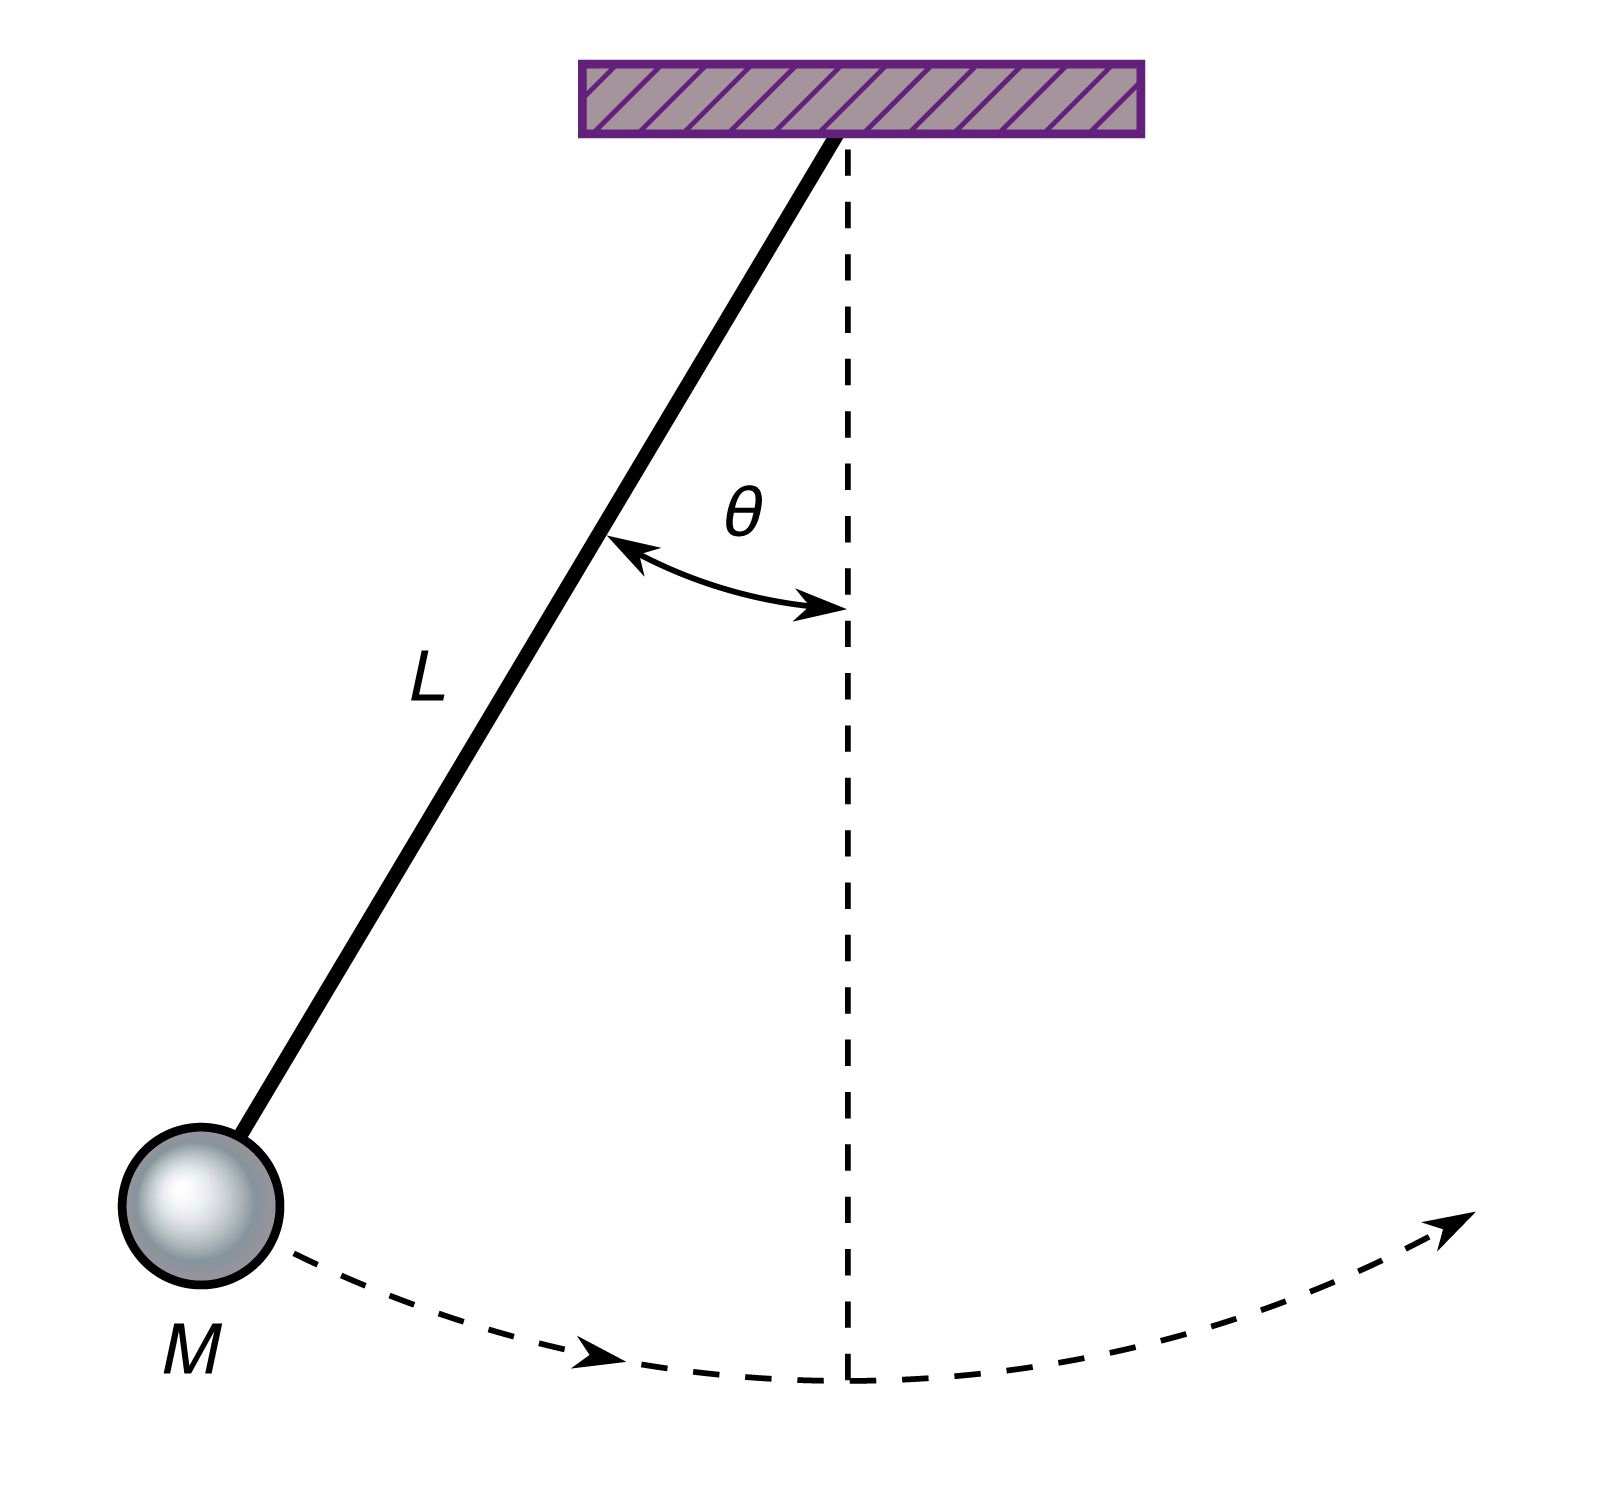
\includegraphics[scale=0.1]{IMG_0200.jpeg}	
		\end{center}
		
		
		
		\vfill
		
		
		
		corso A\\
		Università degli studi di Torino, Torino\\
		4 aprile 2024\\
		
		
	\end{center}
\end{titlepage}
	\tableofcontents
	\newpage
	
	
\end{document}